\chapter{Subjects and Data Preprocessing}
\label{chapter:subjects_perprocessing}
This chapter focuses on ADNI and its study phase ADNI2. The first section briefly describes the history and background of ADNI and our choice of data acquisition   

\section{Subjects}
\label{sec:subjects}
Data used in the preparation of this article were obtained from the Alzheimer\textquoteright s Disease Neuroimaging Initiative (ADNI) database (adni.loni.usc.edu). The ADNI was launched in 2004 by the National Institute on Aging (NIA), the National Institute of Biomedical Imaging and Bioengineering (NIBIB), the Food and Drug Administration (FDA), private pharmaceutical companies and non-profit organizations, as a \$60 million, 5-year public private partnership. The primary goal of ADNI has been to test whether serial magnetic resonance imaging (MRI), positron emission tomography (PET), other biological markers, and clinical and neuropsychological assessment can be combined to measure the progression of mild cognitive impairment (MCI) and early Alzheimer\textquoteright s disease (AD). Determination of sensitive and specific markers of very early AD progression is intended to aid researchers and clinicians to develop new treatments and monitor their effectiveness, as well as lessen the time and cost of clinical trials.

ADNI is the result of efforts of many coinvestigators from a broad range of academic institutions and private corporations, and subjects have been recruited from over 50 sites across the U.S. and Canada. The initial goal of ADNI was to recruit 800 subjects but ADNI has been followed by ADNI-GO and ADNI-2. To date, these three protocols have recruited over 1500 adults, ages 55 to 90, to participate in the research, consisting of cognitively normal older individuals, people with early or late MCI, and people with early AD. The follow up duration of each group is specified in the protocols for the three phases if ADNI: ADNI-1, ADNI-2 and ADNI-GO. Subjects originally recruited for ADNI-1 and ADNI-GO had the option to be followed in ADNI-2. For up-to-date information, see www.adni-info.org.

Although the three studies all aim to advance AD research, there is some differences in participant pools, and adjustments to data collection protocols over time as a result of scientific findings and changing technologies. ADNI2 phase started in January 2011 and ended January 2016. ADNI1 has been a topic of research in our laboratory~\citep{shi2014genetic,zhang2016morphometric} and this motivated us to analyze ADNI2. Participants were recruited across North America during each phase of the study and agreed to complete a variety of clinical assessments. The studies includes participants to make multiple visits but in this study we refrain to baseline and screening data, the marked region in Fig.~\ref{fig:study_schedule}.

\begin{figure}
	\centering
	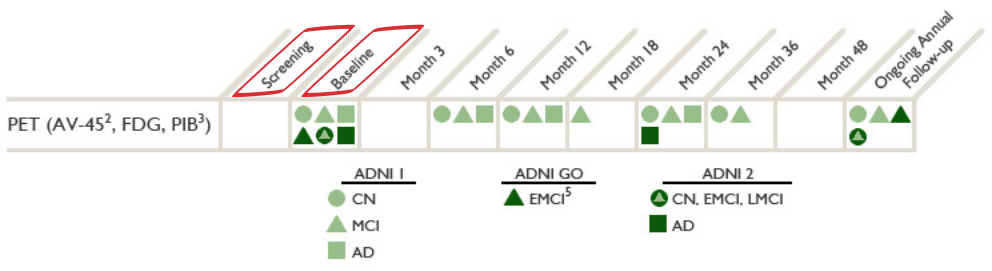
\includegraphics[width=\linewidth]{figures/Imaging_Chart_PET.png}
	\caption[Summary of clinical data and how it is collected.]{The summary of the clinical data for FDG-PET scans ADNI1 is indicated ny light green and the later phases ADNI 2 \& GO are represented by dark green. The typical timeline for image accusation is over 4-5 years and the initial phase is Screening and Baselines. Given the consistency of data for ADNI2 at Baseline we choose the latter for analysis.}
	\label{fig:study_schedule}
\end{figure}
 

\begin{table}
	\centering
	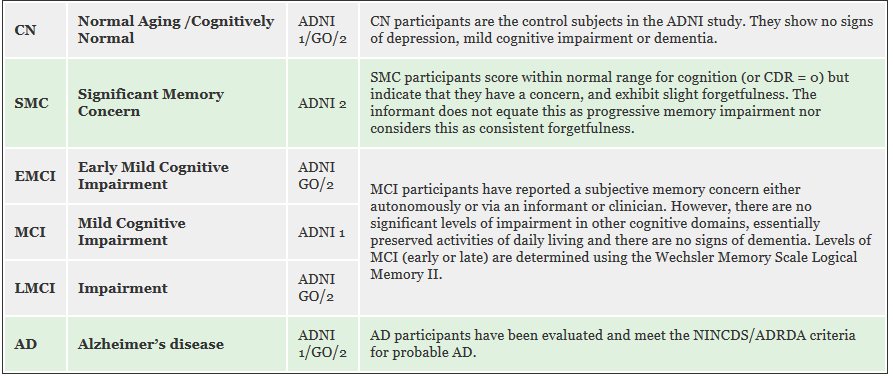
\includegraphics[width=\linewidth]{figures/participant_stages.png}
	\caption[Participant Stages across ADNI 1/GO/2.]{Participant Stages across ADNI 1/GO/2.\footnote{http://adni.loni.usc.edu/study-design/background-rationale/}}
	\label{fig:participant_stages}
\end{table}
  
For this thesis, we studied a total of 668 subjects in the ADNI2 baseline dataset, within this population, there were 146 who had \Alzheimers (AD), 158 had impairment (LMCI), 178 had early mild cognitive impairment (EMCI) and 186 were normal control (CN). Table.~\ref{fig:participant_stages} gives a detailed description of all the stages in disease progression. (SMC) is a new cohort in ADNI 2, it is introduced in the study to minimize the stratification risk among normal control and addressing the gap between healthy elderly controls and Impaired. We choose to ignore (SMC) from our study as the participants with (SMC) suffer from slight forgetfulness and they have a cognitive dementia rating (CDR)~\citep{morris1993clinical} of zero and thus is very loosely based to clinical dementia. 

\section{Data Gathering}
\label{sec:data_gathering}
To acquire \FDGPET data from the ADNI LONI website one has to complete an application process which includes the acceptance of a data user agreement and the submission of and online application form. It is also required that the application includes the institutional affiliation and the proposed research to be conducted using the ADNI data. The image collections are downloaded from the ADNI LONI database at (https://ida.loni.usc.edu). We initially download the image scans across all the accusation stages from the image search engine. We select the uniform pre and post processed scans and download the data in ``NiFTI'' format. Out of $1340$ subjects $774$ were present at baseline and were used in our experimentation.
\begin{figure}[h]
	\centering
	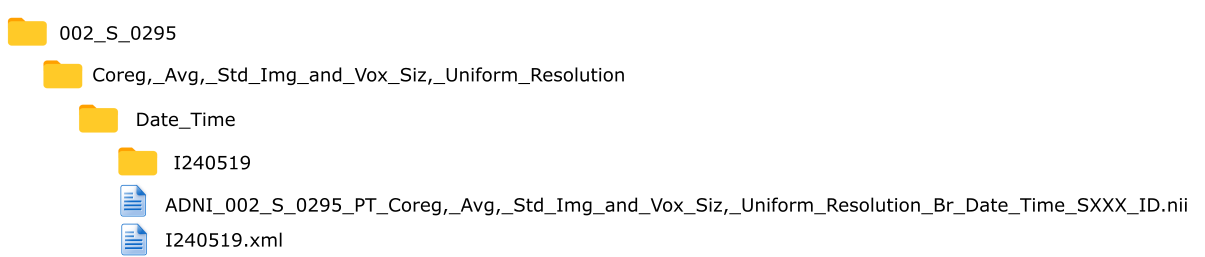
\includegraphics[width=\linewidth]{figures/file_structure}
	\caption[The file structure of downloaded data.]{The file structure of a participant.}
	\label{fig:filestructure}
\end{figure}

\begin{table}[t]
	\begin{center}
		\caption{Demographic information of $668$ studied subjects in ADNI2 baseline dataset.}\label{tab:demographic}
		\begin{tabular}{|P{1.5cm}|P{1cm}P{1cm}P{2.25cm}P{3cm}P{1.25cm}P{1.25cm}P{1.25cm}|}
			\hline
			& Male & Female & Age & Min~/~Max Age & APOE1 & APOE2 & FAQ \\
			\hline\hline
			AD 		& $85$ 	& $61$ & $74.73 \pm 8.15$ 	& $56~/~90$ &	3.11 & 3.63 & 13.39\\
			LMCI 	& $84$ 	& $74$ & $72.5 	\pm 7.5$ 	& $55~/~91$ &	3.03 & 3.54 & 03.62\\
			EMCI 	& $102$ & $76$ & $ 71.3 \pm 7.2 $	& $55~/~89$ &	2.94 & 3.42 & 02.08\\
			CN 		& $89$ 	& $97$ & $ 73.5 \pm 6.25 $ 	& $57~/~89$ &	2.86 & 3.24 & 00.16\\
			\hline
		\end{tabular}
	\end{center}
\end{table}

Fig.~\ref{fig:filestructure} shows the file structure of one participant in the downloaded image collection. Participant is given a subject ID: ``002\_S\_0295'' as shown in Fig~\ref{fig:filestructure}. In the ADNI study after image accusation the \FDGPET ~scans are filtered with a scanner-specific filter function to produce images of a uniform isotropic resolution of 8 mm FWHM. These preprocessed PET data are co-registered, averaged image from their baseline PET scans, which are then reoriented into a standard $160\times160\times96$ voxel image grid, having 1.5 mm cubic voxels. This image grid is oriented such that the anterior-posterior axis of the subject is parallel to the AC-PC line \citep{lee2014parametric}. This standardized image then serves as a reference image for all PET scans on that subject. Fig.~\ref{fig:filestructure} shows the folder name ``Coreg,\_Avg,\_Std\_Img\_and\_Vox\_Siz,\_Uniform\_Resolution'' indicating the type of preprocessing. Additionally a subject may have participated only at the baseline accusation and some other subject may have been involved at both baseline and ADNI-1 year, so a patient may have more than one scan of which we only investigate the baseline one. In Fig~\ref{fig:filestructure} folder ``Date-Time'' has only one record indicating the presence of only one Baseline scan.

Each scan has a unique ID (``I240519'' in Fig.~\ref{fig:filestructure}) and associated to it is a XML file. Form this structure we extract all the XMLs and the NiFTI image scans. To learn about the demographics and segregate the stages in (AD) disease progression we use python to crawl over the XML files. We extract key demographic information from the XMLs and make a dictionary segregating the baseline scans from other visits. From this we form six sets of collections over which we will run our proposed methods. Table.~\ref{tab:demographic} shows the demographic information of the participants.  


\section{Image Preproceessing}
\label{sec:image_preprocessing}
For a patch based method to work on 3D images it requires that a significant portion of the cerebral \FDGPET ~image scan is represented by the generated patches. To minimize the empty and non-essential space in and around the relevant region of interest (ROI), further processing is essential. Fig.~\ref{fig:preprocessing}(a.) shows the data that we immediately get after downloading the \FDGPET ~image scans, as seen in Fig.~\ref{fig:preprocessing}(a.) the scan is surrounded by empty voxels which convey no information and we wish to get rid of it. Before we crop the 3D-image scans we will have to spatially normalize Fig.~\ref{fig:preprocessing}(b.) the image to bring all the scans to a same space. Human brain differs in size and shape and thus goal of spatial normalization is to deform the human brain scans so one subject's brain scans corresponds the same location in another subject's brain scans. To refrain ourself in using only the cerebral ROI we further segmented the scans. Fig.~\ref{fig:preprocessing}(c.) is the normalized and segmented version of our data. 
\begin{figure}[h]
	\centering
	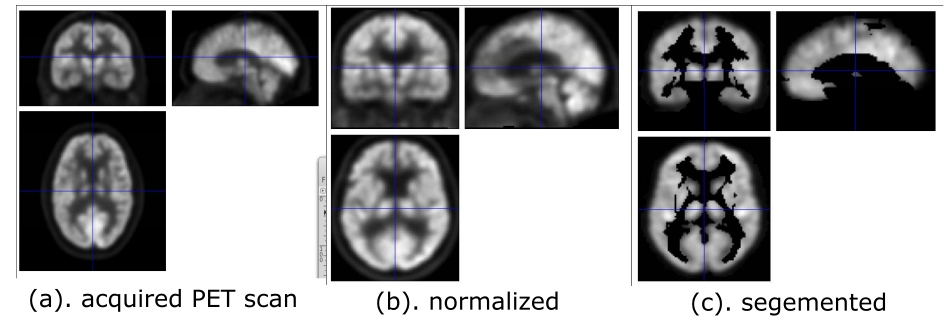
\includegraphics[width=\linewidth]{figures/preprocessing}
	\caption[Prepocessing pipeline.]{Preprocessing pipeline in FDG-PET. (a.) accuired data (b.) aligned \& normalized (c).skull stripped and segemented.}
	\label{fig:preprocessing}
\end{figure}
    
Given a FDG-PET image, the alignment and the image segmentation are automatically performed  software toolkit Statistical Parametric Mapping (SPM12)~\citep{penny2011statistical}\footnote{http://www.fil.ion.ucl.ac.uk/spm/}. Firstly to linearly align all the images into a common space and normalize them we use the (SPM) batch editor. As indicated in Fig~\ref{fig:filestructure} the baseline scans of all the subjects are unique by the image-UID (e.g. ``I240519'') and we can easily mark and distinguish files by this ID. Keeping this in mind we batch normalize and rename the NiFTI files as ``ImageUID.nii'', below is a portion of the .m file created and loaded in to the batch editor for normalization. 
\begin{figure}[h]
	\centering
	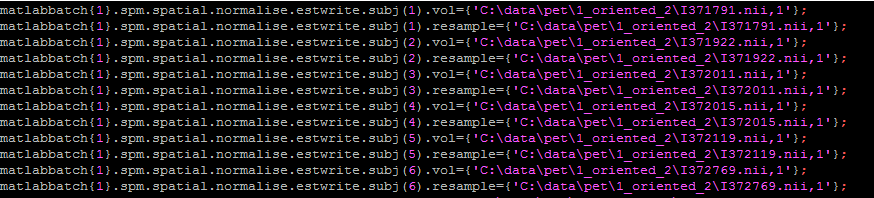
\includegraphics[width=\linewidth]{figures/batching}
	\caption[Code snippet for batching data into spm]{Code snippet for batching data into spm}
	\label{fig:batching}
\end{figure}

Second, we borrow a brain mask from SPM, an AAL template to decide which regions to keep and which to remove. We align the template to the same space as we did to the test images and turn the AAL template (Fig.~\ref{fig:mask}) into a mask by turning all the non-zero voxels to the value of ``1''. Third we compute the dot product of the FDG-PET image scans and the mask generated to segment the region of interest. Keeping the nomenclature of the files consistent with the previous step. Fourth, we conduct spatial smoothing with a Gaussian kernel of the full width at half maximum (FWHM) equal to (8; 8; 8) in three directions (x; y; z).
\begin{figure}[h]
	\centering
	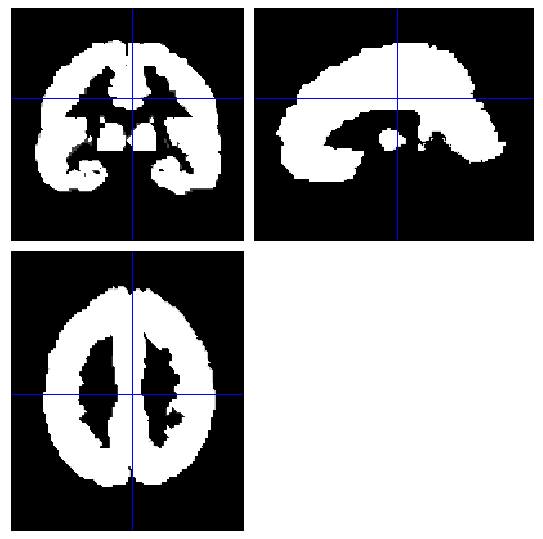
\includegraphics[width=\linewidth]{figures/mask}
	\caption[AAL mask used for segementation]{AAL mask used for segementation}
	\label{fig:mask}
\end{figure}

 
